\chapter{Nanofils}
\label{Chap4}
Muni de ces résultats sur les tests, nous pouvons nous atteler à réaliser le dispositif que nous souhaitions obtenir au départ.
       
    \section{Fabrication}
        %schéma du process flow
        La principale question à se poser est comment, à partir des différentes techniques de salle blanche et des tests effectués, pouvons-nous intégrer les nanofils à une structure que l'on peut caractériser ? Il y a deux types de nanofils, nous détaillerons les différents Process Flow.
        
        \subsection{Jonctions NIS avec nanofils à barrière}
        
        Ici, le but est de réaliser un structure NIS avec les nanofils, le metal normal étant le lead en $Cu$, l'isolant étant la barrière d'$InGaAs$ et le supraconducteur est le nanofil ainsi que le deuxième lead en $Al$.
        
        \begin{figure}
            \centering
            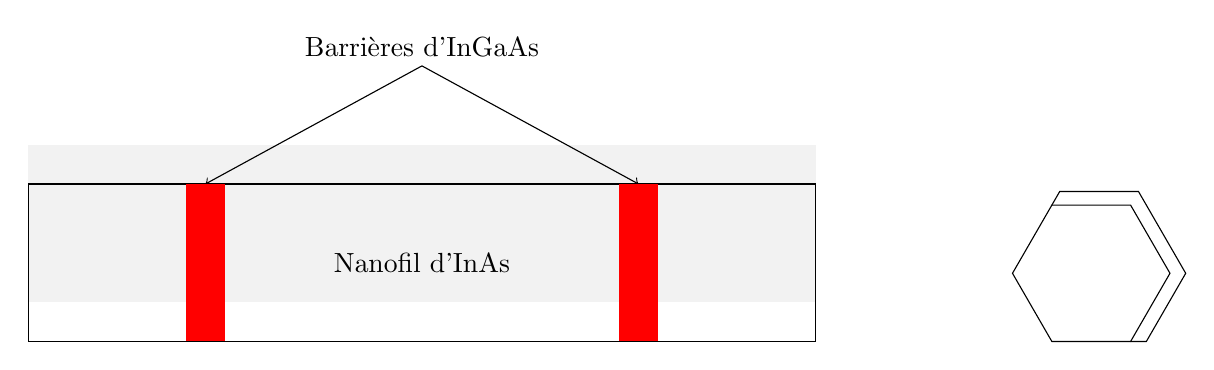
\begin{tikzpicture}
                \fill [color=gray!10] (0,0.5)--(10,0.5)--(10,2.5)--(0,2.5)--cycle;
                \draw (0,0)--(10,0)--(10,2)--(0,2)--cycle;
                \draw [<-] (2.25,2)--(5,3.5);
                \draw [<-] (7.75,2)--(5,3.5);
                \draw (5,3.5)node[above]{Barrières d'InGaAs};
                \draw (5,1) node{Nanofil d'InAs};
                \fill [color=red] (2,0)--(2.5,0)--(2.5,2)--(2,2)--cycle;
                \fill [color=red] (8,0)--(7.5,0)--(7.5,2)--(8,2)--cycle;
                
                \draw (13,0)--++(1,0)--++({cos(60)},{sin(60)})--++({-cos(60)},{sin(60)})--++(-1,0)--++({-cos(60)},{-sin(60)})--cycle;
                \draw (14,0)--++(0.2,0)--++({cos(60},{sin(60)})--++({-1.2*cos(60)},{1.2*sin(60)})--++(-1,0)--++({-0.2*cos(60)},{-0.2*sin(60)});  
            \end{tikzpicture}
            
        \end{figure}
        
        
        
        
    \section{Caractérisation}

    \section{Interpretations}
